\chapter{The Stakeholders}
In this chapter, we will identify the key stakeholders of the project and describe their needs, expectations, and concerns as they relate to the project. By understanding the needs and expectations of our stakeholders, we can ensure that the project meets their requirements and delivers the desired outcomes.
\begin{figure}[ht]
  \centering
  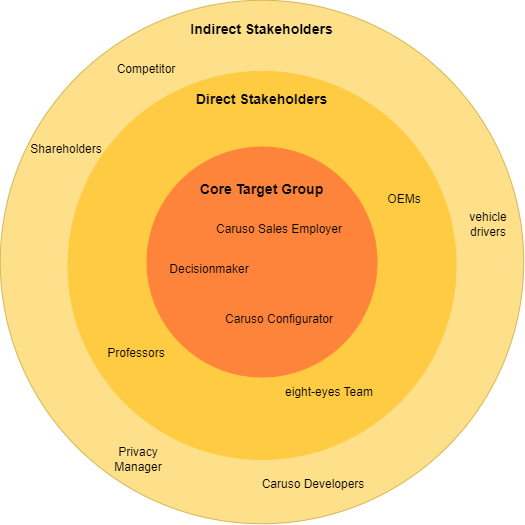
\includegraphics[width=\textwidth]{stakeholders/stakeholders.png}
  \caption{Stakeholders}
  \label{Kap2:Stakeholders}
\end{figure}
Figure \ref{Kap2:Stakeholders} shows the stakeholders of the project. Stakeholders are separated into three categories: the core target group, direct stakeholders and indirect stakeholders. The core target group are the main users Carvis, the people who are intended to use the product. The direct stakeholders are people and organisations who are linked to the project. They either work on the project or provide critical information without which it could not succeed. The indirect stakeholders are people and organisations who also profit from the success of the project but have no bearing on it.

\section{Core Target Group}
The core target group consists of three stakeholders: the Caruso sales employee, the Caruso configurator and the decision maker of a potential customer. The following section will present the obligations of each stakeholder and explain their relevance to the project.

\subsection{The Sales Employee}
The Caruso sales employee is a representative of Caruso who negotiates and enters into contracts with decision makers of other companies and sells them Caruso services. Their obligations include:
\begin{itemize}
  \item the acquisition of customers,
  \item the preparation of sales pitches for decision makers,
  \item the presentation of the sales pitch to build the decision maker's trust in Caruso data,
  \item the answering of any remaining questions the decision maker may have,
  \item the preparation of customer-specific data items,
  \item and the closing of contracts with decision makers.
\end{itemize}
The Caruso sales employee is essential both in the current and the planned future process of acquiring new customers. They were the main point of contact for questions during the design sprints.

\subsection{The Decision Maker}
Decision makers are potential customers of Caruso which are interested in the data provided. They are often the executives of medium-sized companies which hope to improve the workflow in their company or develop new applications using Caruso data. According to Caruso, the most profitable customers are insurances, roadside assistance companies, auto repair shops and fleet management companies. During the design sprints, contact to the decision makers wasn't established directly but their wishes were expressed by the sales employee. Still, their interests are a core driver in the design of the product as it is ultimately intended to convince them to invest in Caruso services. They:
\begin{itemize}
  \item decide whether or not to enter into contracts with Caruso on behalf of their companies,
  \item often have little technical know-how,
  \item and will only buy a product whose value they appreciate and which they trust.
\end{itemize}

\subsection{The Configurator}
The Caruso configurator is an employee which aggregates customer data into an Excel or HTML report. They have technological skill and will prepare the data for sales pitches at the request of the sales employee. Their obligations are:
\begin{itemize}
  \item the aggregation of vehicle data,
  \item the creation of Excel or HTML reports,
  \item and the manual configuration of reports to accommodate a decision maker's individual requests and wishes.
\end{itemize}
After the successful conclusion of this project, the configuration will have a much smaller role or will not be needed at all as Carvis will automatically aggregate the required data and will provide an interface for the sales employee to configure it without needing technical know-how.

\section{Other Stakeholders}
The other stakeholders of the project are the direct and indirect stakeholders. As they are not directly responsible for any requirements of the project, they will not be mentioned in the following chapters and will only briefly be described here.

\subsection{Direct Stakeholders}
\begin{itemize}
  \item \textbf{The eight eyes Team}: The eight eyes team has identified Caruso's wishes and the requirements for an application to fulfil them. This resulting document will provide developers the basis for a successful project.
  \item \textbf{The Professors}: The professors established the first contact to Caruso and organised the central aspects of the project as part of the PSE class.
  \item \textbf{The OEMs}: The OEMs provide the raw vehicle data which Caruso buys and standardises. Without them, this project would not be possible.
\end{itemize}

\subsection{Indirect Stakeholders}
\begin{itemize}
  \item \textbf{The Shareholders}: The shareholders invest in Caruso and thus profit from any new contracts that may be closed as a result of the success of this project.
  \item \textbf{The Competition}: The competition are companies which offer similar services to Caruso. They will be negatively impacted by this projects success.
  \item \textbf{The Drivers}: The drivers are the customers of the decision makers. They will profit if the further use of Caruso data leads to better customer service or new applications they might use.
  \item \textbf{The Caruso Development Team} The development team will expand and maintain the Carvis system in the future.
  \item \textbf{The Data Security Officer}: Data security officers handle the security of Caruso data. Caruso cares about the security of their customer data, however according to Caruso it should not be a priority for the purposes of this project.
\end{itemize}

\section{Personas}
A representative persona has been created for each stakeholder of the core target group to better understand and gain deeper insight into their challenges. These personas include demographic information, a job description, goals, aspirations and challenges they face at work. It also describes how Carvis will support them to overcome their challenges and meet their goals.

\begin{figure}[ht]
  \centering
  \includegraphics*[width=\textwidth]{./Cornelius.pdf}
  \caption{Persona: Sales Employee }
  \label{Persona:Cornelius}
\end{figure}
Figure \ref{Persona:Cornelius} shows "Cornelius von Grünwald" who is representative of the sales employee. As such it is his job to acquire new customers and hold presentations to showcase Caruso data. He has little technical know-how and relies on developers (configurators) to prepare data for him. He prioritises building trust between him and his customers and values their individual wishes.

\begin{figure}[ht]
  \centering
  \includegraphics*[width=\textwidth]{./Rube.pdf}
  \caption{Persona: Decision Maker}
  \label{Persona:Rube}
\end{figure}
Figure \ref{Persona:Rube} shows "Rüdiger Rübe" who is representative of the decision maker of a fleet management company. He is the CEO of a medium-sized taxi company called EuroTaxi. He is interested in expanding his business with innovative technologies, however he needs to first be convinced of their use as every investment is a big risk in terms of time and resources spent. As he  has little technical knowledge and little time, data items need to be presented in a simple and engaging way. 

\begin{figure}[ht]
  \centering
  \includegraphics*[width=\textwidth]{./annie.pdf}
  \caption{Persona: Configurator}
  \label{Persona:Annie}
\end{figure}
Figure \ref{Persona:Annie} shows "Annie Ainsley" who is representative of the configurator. She is a senior Caruso developer who is intimately familiar with the Caruso API and data items. She is often asked by Cornelius to prepare data for him which takes time away for other tasks. She is also not familiar with Rüdiger or other decision makers and can't cater to their wishes well, so she has to be in close contact with Cornelius while she prepares the data for him.